%% Chapter 7 — ML-Assisted State Discrimination
\section{ML-Assisted State Discrimination}
\label{sec:ml}

\subsection{IQ Data and the Discrimination Problem}

Each single-shot readout produces an averaged $(I, Q)$ pair, a point in the
complex plane.  Repeating the preparation and measurement builds up two clouds of
such points, one for $\ket{0}$ and one for $\ket{1}$, whose centroids and spreads
depend on the readout power, resonator parameters, and integration time.  As set
out in Section~\ref{subsec:state_discrim}, for ideal Gaussian clusters of equal
covariance the optimal linear boundary is the LDA hyperplane of
Eq.~\ref{eq:lda_boundary}, the perpendicular bisector of the centroid line after
whitening by the common covariance; QDA relaxes the equal-covariance assumption and gives
a curved boundary.  In practice, state-preparation errors, $T_1$ decay during the
readout pulse, and higher-level leakage ($\ket{2}$, $\ket{3}$) distort the clusters
from ideal Gaussians and motivate more expressive classifiers.  Throughout, we
quote the assignment fidelity of Eq.~\ref{eq:fidelity}, equivalently the average
of the two per-class accuracies.

\subsection{Lightweight Classifiers for FPGA Deployment}
\label{subsec:classifiers}

For eventual on-FPGA deployment, the classifier must be computable using only
fixed-point arithmetic and a small number of multiply-accumulate operations.  Three
constraints matter: latency (the decision must complete in a time negligible next
to the readout window and $T_1$, in practice a few hundred nanoseconds at most, so
as not to extend the readout dead time),
resource usage (it must fit in the available DSP slices and block RAM without
displacing the readout and tProcessor logic), and trainability (it must train on a
laptop from a few thousand calibration shots).

With these constraints in mind, three classifier families are considered.  A
\textbf{linear threshold} (LDA) reduces to a single dot product and a
comparison, the minimum possible arithmetic, directly implementable in the
tProcessor's \texttt{mathi} instruction.  A \textbf{quadratic threshold} (QDA)
evaluates a $2\times2$ matrix product (4 multiply-accumulates) and handles
asymmetric cluster covariances.  A \textbf{small MLP} with inputs $(I, Q)$, one
to three hidden layers of 4–64 neurons with ReLU activations, and a sigmoid output
can be computed as a matrix-vector product and fits in $\lesssim 200$ DSP
slices on the ZCU216.  The following sections report results from evaluating
these classifiers offline on existing experimental data; FPGA deployment is
discussed in Section~\ref{subsec:deployment_path}.  For prior work on
neural-network-based discrimination, including multiplexed multi-qubit readout,
see Lienhard et al.~\cite{Lienhard2022}.

\subsection{Experimental Data}
\label{subsec:ssro_data}

The dataset used throughout this chapter is \texttt{SSRO.h5}, collected on a
superconducting qubit device at Qilimanjaro, and retrieved from a database containing data from past experiments.  It contains 2000 single-shot IQ
measurements per prepared state ($\ket{0}$ and $\ket{1}$).  Each shot is a
single $(I, Q)$ pair, the time-averaged quadrature amplitudes over the readout
window.  The acquisition metadata (qubit type, resonator frequency and linewidth,
readout power, integration window, measured $T_1$) was not stored with the IQ
data; this limits how precisely the synthetic traces of Part~III can be
calibrated, and motivates collecting fully documented raw datasets on the ZCU216.
The class statistics
extracted from this dataset are summarised in Table~\ref{tab:iq_stats}.

\begin{table}[ht]
\centering
\caption{IQ blob statistics extracted from \texttt{SSRO.h5}.}
\label{tab:iq_stats}
\begin{tabular}{lrr}
\toprule
Quantity & $\ket{0}$ & $\ket{1}$ \\
\midrule
Centroid $\mu_I$ (ADU)   & $-0.32$ & $-2.10$ \\
Centroid $\mu_Q$ (ADU)   & $+4.50$ & $+6.31$ \\
Width $\sigma_I$ (ADU)    & $0.649$ & $0.874$ \\
Width $\sigma_Q$ (ADU)    & $0.764$ & $0.967$ \\
IQ separation (ADU)       & \multicolumn{2}{c}{$2.53$} \\
IQ correlation            & $-0.587$ & $-0.664$ \\
\bottomrule
\end{tabular}
\end{table}

The negative IQ correlation in both states indicates a rotated noise ellipse,
consistent with a readout tone that is not perfectly aligned to the I axis.  The
data were split 80/20 into training and test sets (3200 / 800 shots) using
stratified sampling.

\begin{figure}[ht]
  \centering
  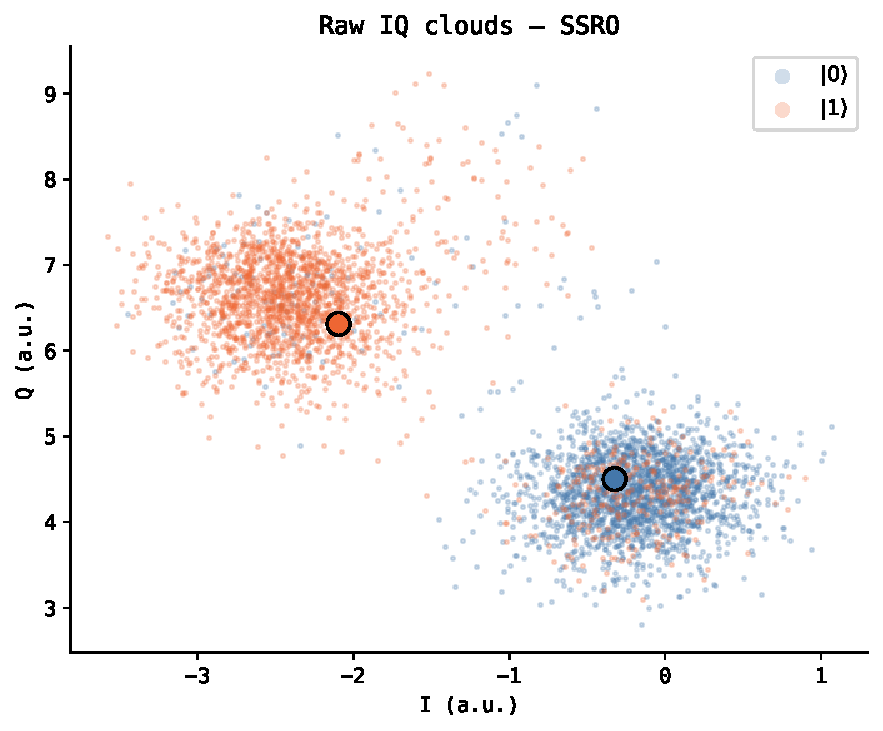
\includegraphics[width=0.55\columnwidth]{code/figures/fig1_iq_scatter}
  \caption{IQ scatter plot of the \texttt{SSRO.h5} dataset (2000 shots per
    state).  Blue: $\ket{0}$; orange: $\ket{1}$.
    Filled circles mark the cluster centroids.  The two clouds are
    well-separated and approximately Gaussian, with the $\ket{1}$ ellipse
    visibly wider, consistent with the $\approx\!1.7\times$ covariance
    asymmetry in Table~\ref{tab:iq_stats}.  The diagonal orientation of both
    ellipses reflects the residual IQ rotation noted in the text.}
  \label{fig:iq_scatter}
\end{figure}

\subsection{Part I: Integrated IQ Discrimination}
\label{subsec:integrated_iq}

LDA, QDA, and a representative MLP (hidden layers 32$\to$16, ReLU) were trained
on the integrated IQ data.  Table~\ref{tab:integrated_results} reports the
assignment fidelity on the held-out test set.

\begin{table}[ht]
\centering
\caption{Assignment fidelity on integrated IQ data (test set, 800 shots).}
\label{tab:integrated_results}
\begin{tabular}{lrrr}
\toprule
Classifier & $\mathcal{F}$ & $\ket{0}$ acc. & $\ket{1}$ acc. \\
\midrule
LDA             & 0.906 & 0.940 & 0.873 \\
QDA             & 0.906 & 0.940 & 0.873 \\
MLP (32$\to$16) & 0.906 & 0.940 & 0.873 \\
\bottomrule
\end{tabular}
\end{table}

All three classifiers achieve identical fidelity, and in fact identical per-class
accuracies: they assign all 800 test shots the same way, because the three decision
boundaries differ
only in regions of the IQ plane that contain no test shots.  The QDA result is the
informative one: the two IQ clouds do \emph{not} share
the same covariance (the
$\ket{1}$ covariance is roughly $1.7\times$ larger than the $\ket{0}$ covariance,
Table~\ref{tab:iq_stats}), so QDA's curved boundary is in principle more expressive
than LDA's linear one.  That it recovers no additional fidelity is explained by the
large cluster separation: the Mahalanobis distance between the centroids is
approximately 2.4, which places the clusters well into the regime where the optimal
boundary is nearly linear regardless of covariance asymmetry.  LDA, QDA, and the MLP
are all saturating the classification capacity of the two-dimensional integrated IQ
input.

The $\ket{0}$ accuracy (94.0\%) exceeds the $\ket{1}$ accuracy (87.3\%),
pointing at a systematic source of $\ket{1}$ misclassification.  This asymmetry
is the first diagnostic signature of $T_1$ relaxation during the readout window,
which causes some $\ket{1}$ shots to produce an integrated IQ that falls in the
$\ket{0}$ blob.

\subsection{Part II: Architecture Search}
\label{subsec:arch_search}

To test whether the LDA–MLP parity in Part I is specific to the (32$\to$16)
architecture, a systematic grid search was performed over 20 MLP configurations
spanning 1–3 hidden layers and 4–64 neurons per layer (17 to 6465 parameters),
evaluated by 5-fold stratified cross-validation.  The LDA baseline quoted here,
$0.898 \pm 0.013$, is the 5-fold CV mean and therefore differs slightly from the
held-out-test value of 0.906 in Table~\ref{tab:integrated_results}.

\begin{table}[ht]
\centering
\caption{Representative architecture grid search results (5-fold CV fidelity);
         see Figure~\ref{fig:grid_search} (Appendix~\ref{appendix:ml}) for all 20
         configurations. LDA baseline:
         $0.898 \pm 0.013$.  No MLP architecture exceeds LDA.}
\label{tab:arch_search}
\begin{tabular}{lrrc}
\toprule
Architecture & $\mathcal{F}$ (CV) & $\pm$ std & $\Delta$ vs.\ LDA \\
\midrule
(4,)         & 0.897 & 0.012 & $-0.001$ \\
(64,)        & 0.897 & 0.012 & $-0.001$ \\
(8, 8)       & 0.896 & 0.012 & $-0.002$ \\
(32, 16)     & 0.897 & 0.012 & $-0.001$ \\
(64, 64)     & 0.897 & 0.012 & $-0.001$ \\
(64, 64, 32) & 0.897 & 0.012 & $-0.002$ \\
\bottomrule
\end{tabular}
\end{table}

The fidelity landscape is flat: no architecture, across three orders of magnitude
in parameter count, improves on LDA.  This is not a failure of the models but a
statement about the data, and it follows directly from Part~I: LDA already finds a
near-Bayes-optimal boundary, and no classifier can improve on it from the same
two-dimensional integrated IQ features.

Further improvement must therefore come from richer inputs, not a more expressive
classifier.  The $\ket{1}$ accuracy deficit diagnosed in Part~I points to the
mechanism: $T_1$ relaxation mid-shot.

\subsection{Part III: Raw-Trace CNN}
\label{subsec:cnn}

\subsubsection{Motivation and the T1 Relaxation Problem}

As established in Section~\ref{subsec:ml_background}, no classifier operating on
integrated IQ can recover a shot in which $T_1$ relaxation occurs mid-window: the
integrator averages over both signal levels and the point lands between the two
clusters, destroying the information about the prepared state.  The raw ADC trace,
by contrast, encodes the relaxation time $t^*$ directly as a step in the IQ
trajectory, and a 1D CNN can detect this step and recover the correct label.
Convolutional filters are suited to exactly this kind of local temporal structure,
which pointwise classifiers cannot exploit.

Demonstrating this directly would require a real dataset of raw ADC traces from a
qubit device, and no such dataset was available for this thesis.  The qubit
processor was not accessible in time, so Parts~I and~II used existing single-shot
IQ data from Qilimanjaro's databases (Section~\ref{subsec:ssro_data}).  That data
is \emph{integrated} IQ, one $(I,Q)$ pair per shot: the per-sample time traces are
discarded on the FPGA, since integrated IQ is the standard readout product, so no
raw traces existed to train on.  Acquiring raw traces
is precisely one of the reasons for setting up the ZCU216 (its
\texttt{acquire\_decimated} mode returns the full time trace); collecting them is
part of the future work this thesis prepares for.

In the meantime, Part~III works with \emph{synthetic} traces.  Here ``synthetic''
does not mean invented: each trace is built from the real device's measured IQ
statistics (the centroids and noise covariances of Table~\ref{tab:iq_stats}) and
shaped into the time-resolved signal a raw acquisition would produce, including the
mid-shot relaxation step.  This lets the full discrimination pipeline, from raw
trace to trained CNN, be developed and validated now, so that it is ready to run on
real traces as soon as a chip is available.

\subsubsection{Synthetic Trace Model}

Each shot is modelled as a noisy cavity response, following the standard
dispersive-readout signal model in which the intracavity field rings up toward its
steady-state value at a rate set by the resonator linewidth
$\kappa$~\cite{Blais2021,Gambetta2007}:
\begin{equation}
  \begin{pmatrix}i(t) \\ q(t)\end{pmatrix}
  = \frac{e(t)}{\bar{e}}\,\boldsymbol{\mu}_{s(t)} + \boldsymbol{\eta}(t),
  \qquad e(t) = 1 - e^{-t/\tau_\text{cav}},
\label{eq:trace_model}
\end{equation}
where $\tau_\text{cav}$ is the ring-up time constant of the envelope, of order
$1/\kappa$ (the field amplitude rings up at $2/\kappa$; on real data
$\tau_\text{cav}$ would be fitted to the measured envelope), and
$\bar{e} = \langle e(t)\rangle_t$ normalises the envelope so that
$\langle(i(t), q(t))\rangle_t = \boldsymbol{\mu}_{s(t)}$, matching the real blob
centroids exactly.  The noise $\boldsymbol{\eta}(t) \sim \mathcal{N}(\mathbf{0},
T\Sigma_s)$ is chosen so that the sample mean has covariance $\Sigma_s$, matching
the real blob widths.  It is drawn independently at each sample; real decimated
traces are low-pass filtered by the DDC, so neighbouring samples are correlated
and step detection on real data is somewhat harder than in this model.

For $\ket{1}$ shots, qubit relaxation is modelled by drawing a relaxation time
$t^*$ from a geometric distribution with rate $1 - e^{-1/T_1}$.  After $t^*$ the
signal switches from $\boldsymbol{\mu}_1$ to $\boldsymbol{\mu}_0$:
\begin{equation}
  \boldsymbol{\mu}_{s(t)} =
  \begin{cases}
    \boldsymbol{\mu}_1 & t < t^* \\
    \boldsymbol{\mu}_0 & t \geq t^*
  \end{cases}.
\end{equation}


\paragraph{Simulation calibration.}
The generator is anchored to the real data through its blob statistics: rectangular
integration of the noiseless traces reproduces the measured \texttt{SSRO.h5}
centroids and widths to within a few percent (the self-consistency check below).
The model is specified in samples; time equivalents assume a \SI{200}{MS/s}
decimated rate, a modelling convention rather than a measured value (the ZCU216's
decimated rate is the ADC rate divided by eight, ${\approx}\SI{307}{MS/s}$ at
\SI{2.4576}{GS/s}).
The relaxation time was set to $T_1 = 600$ samples ($\approx\SI{3.0}{\micro\second}$
at \SI{200}{MS/s}), which gives a relaxation fraction of about 28\% among $\ket{1}$
shots.  This is deliberately larger than on the real device, where the measured
$\ket{1}$ accuracy of 87.3\% implies a much smaller relaxation population; the
synthetic set over-represents mid-readout relaxation as a stress test of the
recovery the CNN is meant to perform.  Recalibrating $T_1$ to the real $\ket{1}$
error rate is left to future work (Section~\ref{sec:conclusions}).  The simulation
parameters are summarised in Table~\ref{tab:sim_params}.

\begin{table}[ht]
\centering
\caption{Synthetic trace simulation parameters.  Blob centroids and widths match
         \texttt{SSRO.h5}; $T_1$ is set to over-represent mid-readout relaxation
         (see text).}
\label{tab:sim_params}
\begin{tabular}{llr}
\toprule
Parameter & Physical meaning & Value \\
\midrule
$T$ & Readout window & 200 samples ($\approx\SI{1}{\micro\second}$) \\
$\tau_\text{cav} \sim \kappa^{-1}$ & Cavity ring-up time constant & 20 samples ($\approx\SI{100}{\nano\second}$) \\
$T_1$ & Qubit relaxation time & 600 samples ($\approx\SI{3.0}{\micro\second}$) \\
Relaxation fraction & $\ket{1}$ shots with $t^* < T$ & $\approx$28\% \\
\bottomrule
\end{tabular}
\end{table}

As a self-consistency check, rectangular integration of the noiseless synthetic
traces reproduces the \texttt{SSRO.h5} centroids to better than 1\% (e.g.\ $\mu_Q$
of $\ket{0}$: $+4.521$ synthetic vs.\ $+4.502$ real) and the cluster widths to a few
percent (e.g.\ $\sigma_I$ of $\ket{1}$: $0.851$ vs.\ $0.874$).

\subsubsection{CNN Architecture and Training}

The \texttt{ReadoutCNN} model operates on raw traces of shape $(T, 2)$.  Two
\texttt{Conv1d} layers (channels $2\!\to\!8$ with kernel 8, stride 2, then
$8\!\to\!16$ with kernel 4, stride 2) compress the time axis, global average pooling
collapses it, and a two-layer dense head ($16\!\to\!16\!\to\!1$) produces the binary
logit for $P(\ket{1})$.  The model has 953 parameters, sized for deployment via
\texttt{hls4ml}~\cite{Fahim2021}, an open-source tool that converts trained neural
networks into FPGA firmware through high-level synthesis.  It was trained for 60
epochs with binary
cross-entropy loss and the Adam optimiser on \num{2000} shots per state, split 80/20
into training and test sets.  The training loss converges smoothly within about 40
epochs and the test fidelity plateaus near 99.75\%, with no sign of overfitting,
consistent with the small model size.

\subsubsection{Results}

Table~\ref{tab:cnn_results} compares LDA on integrated IQ against two classifiers
on the raw traces, evaluated on the same held-out test set (20\%, 800 shots).  The
middle row is the optimal \emph{linear} temporal weighting of the raw samples, a
learned matched filter plus threshold~\cite{Gambetta2007}: an L2-regularised
logistic regression on the flattened $(T,2)$ trace, its regularisation chosen by
cross-validation on the training set.  It reproduces the integrated-IQ result
almost exactly ($\mathcal{F} = 0.819$; 46.7\% on relaxation shots): no linear
weighting represents the nonlinear map from relaxation time $t^*$ to label, so the
CNN's gain comes from its nonlinearity, not merely from seeing more input.

\begin{table}[ht]
\centering
\caption{Classifiers on the synthetic dataset.  LDA operates on the
         time-averaged $(I,Q)$; the logistic regression and the CNN operate on the
         full trace $(T,2)$.
         The synthetic set over-represents relaxation relative to the real device
         (see text), so the LDA fidelity here is lower than the 0.906 of
         Table~\ref{tab:integrated_results}.  All values from the held-out test
         set ($n = 800$; 122 relaxation shots).  The CNN gain row is relative to
         LDA.}
\label{tab:cnn_results}
\begin{tabular}{lrrrr}
\toprule
Classifier & $\mathcal{F}$ & $\ket{0}$ acc. & $\ket{1}$ acc.\ (all) &
             $\ket{1}$ acc.\ (relax.\ only) \\
\midrule
LDA (integrated IQ)  & 0.826  & 0.875 & 0.778 & 0.443 \\
Logistic regression (raw trace) & 0.819 & 0.868 & 0.770 & 0.467 \\
1D CNN (raw trace)   & 0.9975 & 1.000 & 0.995 & 0.984 \\
\midrule
CNN gain             & $+17.1\%$ & $+12.5\%$ & $+21.8\%$ & $+54.1\%$ \\
\bottomrule
\end{tabular}
\end{table}

The CNN classifies the 122 relaxation shots in the held-out test set with 98.4\%
accuracy, against 44.3\% for LDA, a gain of 54.1 percentage points on the shots
that are essentially invisible to integration-based methods.  This confirms the
expectation from Section~\ref{subsec:ml_background}: the CNN exploits the temporal
jump structure of the raw trace rather than merely interpolating between blob
positions.  The $P(\ket{1})$ confidence rises monotonically with relaxation time
$t^*$: shots that relax late in the window (spending most of the trace in
$\ket{1}$) are classified with near-certainty, while shots that relax early
(spending most of the trace in $\ket{0}$) are correctly flagged as ambiguous
(Appendix~\ref{appendix:ml}, Figure~\ref{fig:cnn_confidence}).

These results are simulation estimates anchored to the real device data.  The
synthetic set's relaxation fraction of 28\% is well above the real device, and the
i.i.d.\ noise assumption of the trace model is also favourable (real DDC-filtered
traces carry fewer independent samples), so the headline
17-point fidelity improvement should not be read as the gain expected on real data.
What matters is the qualitative conclusion, and it is robust: a CNN operating on raw
traces has access to temporal information that the rectangular integrator discards,
and this structural advantage persists regardless of the exact $T_1$.  Retraining on
real raw traces, once collected with \texttt{acquire\_decimated}, is the natural
next step (Section~\ref{sec:conclusions}).

\subsection{FPGA Deployment Path}
\label{subsec:deployment_path}

FPGA deployment of the trained classifiers was not attempted here.  This section
outlines the concrete steps required to close the loop
from the trained models to real-time discrimination inside the \QICK{} firmware.

The current readout pipeline (a rectangular integrator followed by the tProcessor
threshold register) already implements LDA implicitly.  Formalising this as an
explicit dot-product instruction (\texttt{mathi}) adds no hardware overhead.  The
CNN requires a separate data path: raw decimated traces from
\texttt{acquire\_decimated} are fed into an \texttt{hls4ml}-synthesised IP block
which, from published \texttt{hls4ml} results on comparably sized
models~\cite{Fahim2021}, is expected to produce a binary decision within
approximately \SI{100}{\nano\second} to
\SI{200}{\nano\second} at \SI{250}{\mega\hertz}, comfortably inside the
few-hundred-nanosecond latency budget of Section~\ref{subsec:classifiers}.

The full deployment sequence is:
\begin{enumerate}
  \item \textbf{Collect real raw traces}: connect the ZCU216 to a qubit chip and
        acquire \texttt{SSRO\_raw.h5} with \texttt{acquire\_decimated} (shape
        $(2, N_\text{shots}, T, 2)$), setting \texttt{readout\_length} to at least
        $3/\kappa$ to capture the full cavity ringdown.
  \item \textbf{Retrain and validate}: retrain on real traces, calibrating the
        synthetic $T_1$ to the measured $\ket{1}$ error rate so the synthetic set
        can supplement the real data.
  \item \textbf{Export to HLS}: convert the trained model (PyTorch~$\to$~ONNX) with
        \texttt{hls4ml}~\cite{Fahim2021}, targeting the ZCU216 fabric
        (\texttt{xczu49dr}), \texttt{io\_stream}, and \texttt{ap\_fixed<16,6>}
        precision.
  \item \textbf{Synthesise and integrate}: build the HLS project in Vivado and add
        the IP block to the QICK bitstream alongside the existing readout chain.
  \item \textbf{Benchmark}: compare LDA-threshold, CNN-IP, and host-side
        discrimination on the same data to quantify the latency and fidelity gains.
\end{enumerate}

Based on the model's 953 parameters and typical \texttt{hls4ml} resource scaling
for comparable architectures, the CNN IP block is expected to require on the order
of \num{10000} LUTs and tens of DSP slices, a small fraction of the ZCU216's
available fabric, though this must be confirmed by synthesis.
